\documentclass[a4paper,12pt]{article}
%\usepackage[utf8]{inputenc}
\usepackage{enumerate,amssymb,amsthm,multicol,epsfig,dsfont}
\usepackage{multirow}
\usepackage{longtable}
\usepackage{booktabs}
\usepackage{graphicx}
\usepackage{amsmath}
%\usepackage{multicol}
\theoremstyle{definition}

\newtheorem{example}{Example}
\newtheorem{question}{Question}
\newtheorem{theorem}{Theorem}
\newtheorem{definition}{Definition}
\newtheorem{problem}{Problem}
\textwidth=6.5in
\oddsidemargin=-0.25in
\textheight=9.25in
\voffset=-0.375in


\newcommand{\IR}{\mathbb{R}}
\newcommand{\IC}{\mathbb{C}}
\newcommand{\IF}{\mathbb{F}}
\newcommand{\IQ}{\mathbb{Q}}
\newcommand{\IZ}{\mathbb{Z}}
\newcommand{\IN}{\mathbb{N}}
\newcommand{\CL}{\mathcal{L}}
\newcommand{\CN}{\mathcal{N}}
\newcommand{\CR}{\mathcal{R}}
\newcommand{\CS}{\mathcal{S}}


%\newcommand{\mod}{\mathrm{mod }}
\renewcommand{\iff}{\textbf{iff}}
\newcommand{\ie}{that is, }
\newcommand{\norm}[1]{\|#1\|}
\newcommand{\inner}[1]{\langle#1\rangle}
\newcommand{\RT}{\mathrm{T}}

\begin{document}
\begin{minipage}[t]{\textwidth}%
  \centering
{\textbf{DA-IICT, Gandhinagar}}\par
  {\textbf{Lecture Notes}} \par
{\textbf{Subject: Probability, Statistics and Information Theory (SC222)}}
\end{minipage}
\par
\bigskip
\begin{minipage}[t]{.7\textwidth}%
  \textbf{Date: \underline{23/01/2021}} \par
  \textbf{~} \par
  \textbf{Name: Dhameliya Sanny Gobarbhai} \par
\end{minipage}%
\hfill
\begin{minipage}[t]{.4\textwidth}%
  \textbf{Reg. No.: 201901031} \par
  \textbf{~} \par
  \textbf{Lecture No.: 3} \par

\end{minipage}
\vskip 0.5cm
\hrule
\thispagestyle{empty}
\vskip 1.0cm
\section*{Introduction}
\par  These notes is cover some impotent topic of probability,like as Sample Space and event,Axiomatic approach for define probability,conditional probability and Important theorems like total probability theorem and bayes' theorem.
\section {Sample Space and Event}
\textbf{\underline{Sample Space :-}}  
\vskip 0.25cm
\par Let's do any experiment or process we get  all possible outcomes,then take a union set of all possible outcomes is call Sample Space.\\
\par we define Sample Space by $\Omega$ notation.
\vskip 0.25cm
\par we take any of the event from Sample Space.we define the probability of this event from 0 to 1 .when summing all the probability of the event of the sample space is should be equal to 1. \\
\par\begin{center}
       $\sum_{E\in \Omega}{P(E)}=1 $\\
       \end{center}\par
\par  Probability of  Universal Facts is 1 and NULL event is 0.\\
\vskip 0.25cm
Example :
\par Sun is rise in east, it's probability is 1 (Universal Fact).\par
Sun is rise in west, it's probability is 0 (Null event).\\
\vskip 0.25cm
Example :
\par Let's take Sample Space S $=\{A,B,C\}$. The Probability P(A) $=\frac{1}{2}$,
 P(B) $=\frac{1}{3}$ and \\
P(C) $=\frac{1}{6}$.
\vskip 0.5cm

\par hear we take sum of all event,which is belong into our Sample Space  when sum of all this event probability is equal to 1.\\
   \begin{center}
        $ P(A)+P(B)+P(C)=1 $ 
   \end{center}
\par if all event of any sample space which have equally probable it is called uniform probability distribution.
\vskip 0.25cm
Example :
\par suppose we have a dice when we it filliped down then all possible outcome
is $\Omega= $ $\{1,2,3,4,5,6\} $
\vskip 0.5cm
\par hear we get any number on dice is equally likely .it Menes we get any number from 1 to 6 on dice is equal probability is $\frac{1}{6}.$ 

\section {Axiomatic Approach for Defining Probability}
\par Axiomatic probability is a unifying probability theorem. hear we take any of sample space of any random experiment and also we define probability  is a set of function of P.so,
  \begin{center}
      $ P : \Omega \to [0 , 1] $
  \end{center}
\par function of probability is satisfying three of axioms:\\
\vskip 0.25cm
\par (I) Let's take any event from the sample space, the Probability of this event is greater or equal to zero ( NON ZERO valued ).
         \begin{center}
             $P(E)\geq 0 $
         \end{center}\\
         
          hear E is denoted any event from Sample Space $\Omega $.\\
\par (II) when $\Omega $ is denoted sample space such that $ P(\Omega) = 1 $
and also the probability of any of outcome or event happening is one Hundred parent.\\
\par (III) In sample space we take event's  as like $ E_1,E_2,E_3....$ is a countable infinite collection of mutually exclusive event's $(E_i \cap E_j = \phi , \forall{i}\neq{j})$ then
          \begin{center}
              $P( \cup_{i=1}^{\infty} E_i ) = \sum_{i=1}^{\infty} P( E_i )$
          \end{center}\\
\par hear also noted if union set of all event which is belonging to in sample space $\Omega$ is equal to sample space then this type of  countable collection of event is called exhaustive.
                 \begin{center}
              $ \cup_{i=1}^{\infty} E_i  = \Omega$
          \end{center}\\  
\par hear both condition is satisfy so it's called mutually exclusive and exhaustive event.\\
\\
\textbf{\underline{}}\textbf{Mutually Exclusive} \textbf{\textbf{:-}} \\
\par hear any of two event in sample space  $\Omega $ ,Let's take any event A and B such that , event A and B is called Mutually Exclusive if it Menes 
$A \cap B = \phi $
 \begin{center}
     $P(A \cup B) = P(A) + P(B) $
\end{center}\\
it Menes A and B is Mutually exclusive then the probability of A or B is  equal to probability of A and sum of probability of B. \\
\vskip 0.25cm
Example :
\par suppose we have a coin and  we flip it coin for three time's. then we give many of outcomes, hear we assuming for all outcomes it is equally likely then find the probability for below events.
\vskip 0.5cm
\par hear when we flip coin for three time's we get  different 8 outcomes.which we define in our sample space.\\
 \begin{center}
    $\Omega =\{HHH,HTH,THH,TTH,HHT,HTT,THT,TTT \} $  
 \end{center}\\
\Par $\ E_1 : $ The event that third time's we get head ?\\
\par $\ E_1 =\{HHH,HTH,THH,TTH\} $\\
\begin{center}
    $ P[E_1] = \frac{4}{8} = \frac{1}{2}$
\end{center}\\
\Par $\ E_2 : $ The event that at least two of the tail ?\\
\par $\ E_2 =\{TTH,HTT,THT,TTT\} $\\
\begin{center}
    $ P[E_2] = \frac{4}{8} = \frac{1}{2}$
\end{center}\\ 
\Par $\ E_3 : $ The event that all outcome is equally (all are H or all are T) ?\\
\par $\ E_3 =\{HHH,TTT\} $\\
\begin{center}
    $ P[E_3] = \frac{2}{8} = \frac{1}{4}$
\end{center}\\
\vskip 0.25cm\\
Example :
\par suppose we have a beg ,when we shown in side the beg their have 15 orange ball, 12 yellow ball,3 red ball and 4 green ball. in a one try you will select any of 5 ball's.then find the probability  of given below.\\
\vskip 0.5cm\\
\par we have total ball is 15 + 12 + 3 + 4 = 34. \\
\\ 
\Par $\ E_1 : $ the event that each of ball is orange ?\\
\begin{center}
    $ P[E_1] = \frac{^{15}C_5}{^{34}C_5} $
\end{center}\\
\Par $\ E_2 : $ the event such that one red and 4 orange ball ?\\
\begin{center}
    $ P[E_2] = \frac{(^{3}C_1)*(^{15}C_4)}{^{34}C_5} $\\
\end{center}\\
\Par $\ E_1 : $ the event such that 2 green 2 yellow and one red ?\\
\begin{center}
    $ P[E_1] = \frac{(^{4}C_2)*(^{12}C_2)*(^{4}C_1)}{^{34}C_5} $\\
\end{center}\\
\section{Conditional Probability}
Let's take two event $E_1  and E_2$ which is laying into sample space such that 
outcomes or event $ E_2 $ it is depended on previous outcome or event $ E_1 $ . Then it is denoted by $P(\frac{E_2}{E_1})$ .\\
\begin{center}
    $ P(\frac{E_2}{E_1}) = \frac{P(E_1\cap E_2)}{P(E_1)} $   $ (P(E_1)\neq{0}) $
\end{center}
\textbf{\underline{Notes :-}}\\
\par (I) $P(\frac{E_2}{E_1})\geq{0}$\\
\par (II) $P(\frac{E_1\cup E_2}{F}) = P(\frac{E_1}{F}) + P(\frac{E_2}{F}) $\\
\Par hear $E_1$ and $E_2$  is mutually exclusive event,it Menes $E_1 \cap E_2 = \phi $.\\
\par(III) $P(\frac{E\cap \Omega}{E}) = P(\frac{E}{E}) = 1$\\
\vskip 0.25cm\\
Example :
\par Suppose we have have a dies. we flip it for three time then, let's considered two event E and F.event E is denoted third time we get number 4 on dies.and event F denoted first two time's we get 6 and 5.then find the probability of event E when give event F.(Hint : find probability P($\frac{E}{F}$) ).
\vskip 0.5cm\\
\par when flip the dies for three time then get total outcomes is equal to 216.\\
\par F: we get 6 and 5 number on first two time's, so total outcomes it is 6.\\
\par so, total probability is $P(F)=\frac{6}{216} = \frac{1}{36}$\\
\par $E \cap F$ : we get number 4 when first two times get number is 6 and 5 is equal to 1.\\
\par so, total probability is $P(E \cap F)=\frac{1}{216}$\\
\par then  $ P(\frac{E}{F}) = \frac{P(E\cap F)}{P(F)} =\frac{\frac{1}{216}}{\frac{6}{216} } =(\frac{1}{6})$\\
\vskip 0.25cm\\
\section{Independent Event}
\par Let's take two event from sample space A and B.hear event A and B is called independent event  if the probability of both happen is the product of the probability that first happen and the probability of second happen then,\\
  \begin{center}
      $P(A \cap B) = P(A)*P(B) $\\
 \end{center}
\par hear, three type's of Associates :\\
\par (I) Negative Associated :\\
    \begin{center}
      $P(A \cap B) <  P(A)*P(B) $\\
     \end{center}
\par (II) Positive Associated :\\
     \begin{center}
      $P(A \cap B) >  P(A)*P(B) $\\
     \end{center}
\par (III) independent event :\\
    \begin{center}
     $P(A \cap B) =  P(A)*P(B) $\\
    \end{center}
     \begin{center}
     $P(\frac{A}{B}) = p(A) $ \\
    \end{center}
     \begin{center}
    \par $P(\frac{B}{A})= P(B) $\\
    \end{center}
\vskip 0.25cm\\
Example:
\par suppose we have 52 card's.and we have take one of the card from their.let's consider two event E and F from their.hear event E denoted chosen card is hearts
and event F is denoted chosen card is aces.\\
\vskip 0.5cm\\
\par  total number of card is 52.\\
\par event E: chosen card is hearts,for that total outcome is equal 13.\\
\begin{center}
       $P(E)=\frac{13}{52}=\frac{1}{4}$\\
\end{center}
\par event F: chosen card is aces,for that total outcome is equal 4.\\
\begin{center}
       $P(F)=\frac{4}{52}=\frac{1}{13}$\\
\end{center}
\par event of both $(E \cap F)$ : chosen card is heart and also it is ace for that total outcome is equal 1.
\begin{center}
       $P(E \cap F)=\frac{1}{52}$\\
\end{center}
\par then,
\begin{center}
          $ P(\frac{E}{F}) = \frac{P(E\cap F)}{P(F)} = \frac{\frac{1}{52}}{\frac{1}{13} } =(\frac{1}{4}) = P(E)$
\end{center}
\par so,hear above equation is denoted independent Event.
\section{Total Probability Theorem}\\
\par Let's take sample space $\Omega $ and divide into the set of ${E_1,E_2,E_3,......E_n}.$ Suppose every event $E_1,E_2,....E_n $ has probability which is Non-Zero.Let's take any event A such that,
\vskip 0.20cm
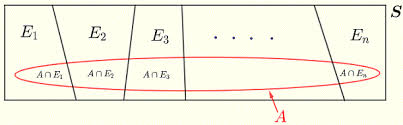
\includegraphics[width=\linewidth]{
proba.jpg}\par
\\
%\begin{center}
    $P(A) = P(E_1)*P(\frac{A}{E_1}) + P(E_2)*P(\frac{A}{E_2}) + P(E_3)*P(\frac{A}{E_3}) +..........+ P(E_n)*P(\frac{A}{E_n})\\
\par = \sum_{j=1}^{n}{P(E_j)*P(\frac{A}{E_j})} $\\
\par hear $E_i \cap E_j = \phi ,\forall{i}\neq{j}$\\ 
\par so this is mutually exclusive  event's for every pair of sample space.\\
\par $ S = E_1 \cup E_2 \cup E_3 ......\cup E_n $ \\
\vskip 0.25cm\\
Example :
one parson promise for particular work of construction.Probability of strike occurs during work is 0.65 . if strike don't occur then probability of finishing construction work is 0.80 and if strike occur then probability of finishing work in time is 0.32 then find the probability of finishing construction in time. 
\vskip 0.5cm
\par hear, event A is denoted finishing construction in time,it's probability is P(A).\\
\par event $E_1$ is denoted strike is occur ,it's probability is P( $E_1$) = 0.65\\
\par event $E_2$ is denoted strike don't occur ,it's probability is P( $E_2$)=0.35\\
\par if strike don't occur and also finishing construction work ,it's probability is P($\frac{A}{E_1}$)=0.80\\
\par if strike is occur and also finishing construction work ,it's probability is P( $\frac{A}{E_2}$)=0.32\\
\\
\par at least,
\par total probability of finishing construction  work at time is,
\begin{center}
      $ P(A) = P(E_1)*P(\frac{A}{E_1}) + P(E_2)*P(\frac{A}{E_2})
            = (0.65)*(0.80)+(0.35)*(0.32)
            = 0.632 $
\end{center}
\section{Bay's Theorem}\\
\par Let's take the sample space $ \Omega $ and divide into Mutual Exclusive event ${E_1,E_2,E_3........E_n}$ such that $ S = E_1 \cup E_2 \cup E_3 ......\cup E_n $ and A is non zero event.\\
\par so,
\begin{center}
    $P(\frac{E_i}{A}) = \frac{P(E_i \cap A )}{P(A)} = \frac{P(E_i) * P(\frac{A}{E_i})}{\sum_{j=1}^{n}{P(\frac{A}{E_j})}} $
\end{center} 
\vskip 0.25cm
Example :
\par Suppose we have three box's each of them has two coins.first of box has two has two coins first of box has two gold coin.second box has two silver coins and third box has one silver coins and  one gold coin.if manan is chosen any box randomly and take a coin.find the probability if chosen box has a gold  coin  then second coin is also gold.
\vskip 0.5cm\\
\par for simplicity let's considered tree diagram  which is given below (tree method to find a probability).\\
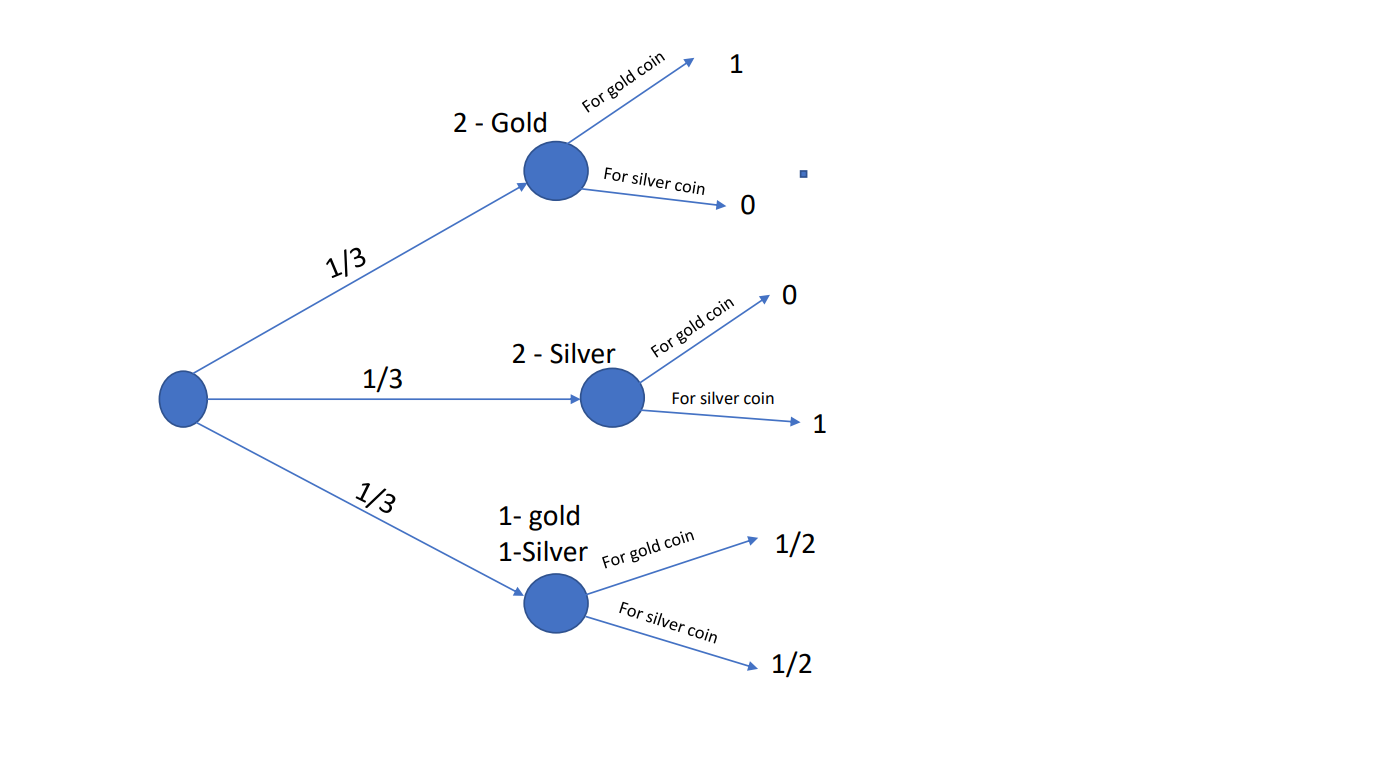
\includegraphics[width=\linewidth]{
treeprob.png}\par
%\par Let's considered a  
\par hear let's consider any event E which is denoted chosen box has second coin is gold coin and event A is denoted first coin is also gold coin then it's probability is,\\
\begin{center}
      $P(E \cap A) = 1 *(\frac{1}{3}) = \frac{1}{3}$
\end{center}\\
\par chosen box has first coin is gold coin it's total probability is\\

      $ P(A) = P(E_1)*P(\frac{A}{E_1}) + P(E_2)*P(\frac{A}{E_2}) + P(E_1)*P(\frac{A}{E_1}) = 1*(\frac{1}{3}) + 0*(\frac{1}{3}) +(\frac{1}{2})*(\frac{1}{3}) $\\
\par $ = \frac{1}{3} + 0 + \frac{1}{4} = \frac{7}{12}$
\\
\par by the Bay's Theorem,
\begin{center}
       $ P(\frac{E}{A}) = \frac{P(E \cap A)}{P(A)} = \frac{\frac{1}{3}}{\frac{7}{12}} = \frac{4}{7} $

\end{center}







    
















 



 





 








\end{document}
